

%% AP Physics MC Questions Archive
%%----------------------------------------


%% First Law Tension
%%----------------------------------------
\element{ap}{
\begin{question}{first-law-tension-q01}
    Two massless strings of equal length are used to suspend a ball as shown above.
    \begin{center}
    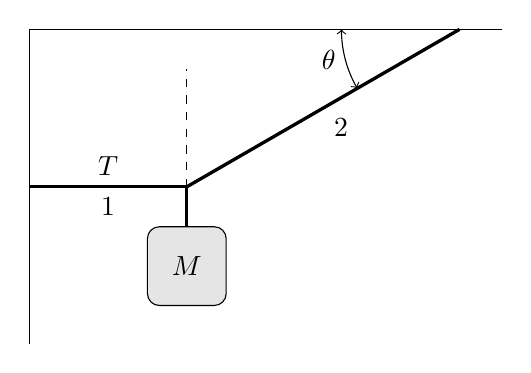
\begin{tikzpicture}
        %% Nodes
        \coordinate (A) at (0,0);
        \coordinate (B) at (+5.464,0);
        \coordinate (C) at (2,-2);
        \coordinate (D) at (0,-2);
        %% Lines
        \draw (0,0) -- (6,0);
        \draw (0,0) -- (0,-4);
        \draw[very thick] (B) --  (C) node[pos=0.5,anchor=north west] {2};
        \draw[very thick] (C) --  (D) node[pos=0.5,anchor=south] {$T$};
        \draw[very thick] (C) --  (D) node[pos=0.5,anchor=north] {1};
        \draw[dashed] (C) -- ++(90:1.5);
        \draw[<->] (B) ++ (210:1.5) arc (210:180:1.5) node[pos=0.5,anchor=east] {$\theta$};
        %% Mass
        \node[draw,fill=white!90!black,rectangle,rounded corners=1ex,minimum size=1cm,anchor=north,yshift=-0.5cm] (M) at (C) {$M$};
        \draw[very thick] (M.north) -- (C);
    \end{tikzpicture}
    \end{center}
    If the tension in the first string is $T$,
        what is the tension in the second string?
    \begin{multicols}{2}
    \begin{choices}
        \wrongchoice{$T\sin\theta$}
        \wrongchoice{$T\cos\theta$}
      \correctchoice{$\dfrac{T}{\cos\theta}$}
        \wrongchoice{$mg - T$}
        \wrongchoice{$mg - T\sin\theta$}
    \end{choices}
    \end{multicols}
\end{question}
}

\element{ap}{
\begin{question}{first-law-tension-q02}
    A box of mass \SI{50}{\kilo\gram} is held by two identical,
        vertical, and massless ropes.
    What is the tension in each string?
    \begin{multicols}{3}
    \begin{choices}
        \wrongchoice{\SI{50}{\newton}}
      \correctchoice{\SI{250}{\newton}}
        \wrongchoice{\SI{500}{\newton}}
        \wrongchoice{\SI{300}{\newton}}
        \wrongchoice{\SI{100}{\newton}}
    \end{choices}
    \end{multicols}
\end{question}
}

\newcommand{\apFirstLawTensionQThree}{
\begin{tikzpicture}
    %% Ceiling
    \node[anchor=south,fill,pattern=north east lines,minimum width=4cm, minimum height=0.05cm] at (0,0) {};
    \draw (-2,0) -- (2,0);
    %% Block
    \node[draw,fill=white!90!black,rectangle,rounded corners=1ex,minimum size=1cm,anchor=north,yshift=-0.5cm] (M) at (0,-1) {$M$};
    %% Rope
    \draw[ultra thick] (M.north) -- (0,0);
\end{tikzpicture}
}

\element{ap}{
\begin{question}{first-law-tension-q03}
    A uniform rope weighing \SI{30}{\newton} hangs from a ceiling as shown below.
    \begin{center}
        \apFirstLawTensionQThree
    \end{center}
    A box of weight \SI{50}{\newton} hangs from the rope.
    What is the tension in the rope?
    \begin{choices}
        \wrongchoice{\SI{50}{\newton} throughout the rope.}
        \wrongchoice{\SI{65}{\newton} throughout the rope.}
        \wrongchoice{\SI{80}{\newton} throughout the rope.}
      \correctchoice{It varies from \SI{50}{\newton} at the bottom of the rope to \SI{80}{\newton} at the top.}
        \wrongchoice{It varies from \SI{80}{\newton} at the bottom of the rope to \SI{50}{\newton} at the top.}
    \end{choices}
\end{question}
}

\element{ap}{
\begin{question}{first-law-tension-q04}
    A uniform rope weighing \SI{30}{\newton} hangs from a ceiling as shown below.
    \begin{center}
        \apFirstLawTensionQThree
    \end{center}
    A uniform rope of weight \SI{60}{\newton} hangs from a ceiling as shown below.
    A box of weight \SI{90}{\newton} hangs from the rope.
    What is the ratio of the tension at the top of the rope to the tension at the bottom?
    \begin{multicols}{3}
    \begin{choices}
        \wrongchoice{\num{2/5}}
        \wrongchoice{\num{2/3}}
        \wrongchoice{\num{1}}
        \wrongchoice{\num{3/2}}
      \correctchoice{\num{5/3}}
    \end{choices}
    \end{multicols}
\end{question}
}

\newcommand{\apFirstLawTensionQFive}{
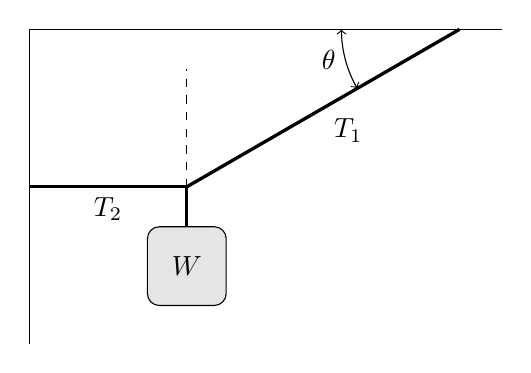
\begin{tikzpicture}
    %% Nodes
    \coordinate (A) at (0,0);
    \coordinate (B) at (+5.464,0);
    \coordinate (C) at (2,-2);
    \coordinate (D) at (0,-2);
    %% Lines
    \draw (0,0) -- (6,0);
    \draw (0,0) -- (0,-4);
    \draw[very thick] (B) --  (C) node[pos=0.5,anchor=north west] {$T_1$};
    \draw[very thick] (C) --  (D) node[pos=0.5,anchor=north] {$T_2$};
    \draw[dashed] (C) -- ++(90:1.5);
    \draw[<->] (B) ++ (210:1.5) arc (210:180:1.5) node[pos=0.5,anchor=east] {$\theta$};
    %% Mass
    \node[draw,fill=white!90!black,rectangle,rounded corners=1ex,minimum size=1cm,anchor=north,yshift=-0.5cm] (M) at (C) {$W$};
    \draw[very thick] (M.north) -- (C);
\end{tikzpicture}
}

\element{ap}{
\begin{question}{first-law-tension-q05}
    %% Base your answers to questions 5 and 6 on
    The diagram below shows an object of weight $W$ suspended from two massless strings.
    \begin{center}
        \apFirstLawTensionQFive
    \end{center}
    The tension in string $T_1$ is:
    \begin{multicols}{2}
    \begin{choices}
        \wrongchoice{$W$}
        \wrongchoice{$W\sin\theta$}
      \correctchoice{$\dfrac{W}{\sin\theta}$}
        \wrongchoice{$W\cos\theta$}
        \wrongchoice{$\dfrac{W}{\cos\theta}$}
    \end{choices}
    \end{multicols}
\end{question}
}

\element{ap}{
\begin{question}{first-law-tension-q06}
    %% Base your answers to questions 5 and 6 on
    The diagram below shows an object of weight $W$ suspended from two massless strings.
    \begin{center}
        \apFirstLawTensionQFive
    \end{center}
    The tension in string $T_2$ is:
    \begin{multicols}{2}
    \begin{choices}
        \wrongchoice{$W\cos\theta$}
        \wrongchoice{$\dfrac{W}{\cos\theta}$}
      \correctchoice{$\dfrac{W}{\tan\theta}$}
        \wrongchoice{$W\tan\theta$}
        \wrongchoice{$W\sin\theta$}
    \end{choices}
    \end{multicols}
\end{question}
}

\element{ap}{
\begin{question}{first-law-tension-q07}
    A uniform rope of weight \SI{50}{\newton} hangs from a ceiling.
    A box hangs from the bottom of the rope.
    The ratio of tension at the top of the rope to the tension at the bottom is $3:1$.
    What is the mass of the box?
    \begin{multicols}{2}
    \begin{choices}
        \wrongchoice{\SI{100}{\kilo\gram}}
        \wrongchoice{\SI{50}{\kilo\gram}}
        \wrongchoice{\SI{20}{\kilo\gram}}
        \wrongchoice{\SI{10}{\kilo\gram}}
      \correctchoice{\SI{2.5}{\kilo\gram}}
    \end{choices}
    \end{multicols}
\end{question}
}

\element{ap}{
\begin{question}{first-law-tension-q08}
    A ball of mass $m$ hangs vertically from a massless string experiencing a tension $T$.
    What force is required to pull the ball out to an angle $\theta$ from the vertical?
    \begin{multicols}{2}
    \begin{choices}
        \wrongchoice{$mg\sin\theta$}
        \wrongchoice{$mg\cos\theta$}
      \correctchoice{$mg\tan\theta$}
        \wrongchoice{$2mg\tan\theta$}
        \wrongchoice{$\dfrac{mg}{cos\theta}$}
    \end{choices}
    \end{multicols}
\end{question}
}

\element{ap}{
\begin{question}{first-law-tension-q09}
    Base your answer to the following question on the diagram below.
    \begin{center}
    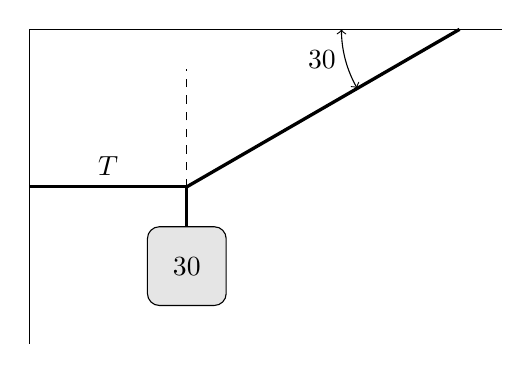
\begin{tikzpicture}
        %% Nodes
        \coordinate (A) at (0,0);
        \coordinate (B) at (+5.464,0);
        \coordinate (C) at (2,-2);
        \coordinate (D) at (0,-2);
        %% Lines
        \draw (0,0) -- (6,0);
        \draw (0,0) -- (0,-4);
        \draw[very thick] (B) --  (C) node[pos=0.5,anchor=north west] {};
        \draw[very thick] (C) --  (D) node[pos=0.5,anchor=south] {$T$};
        \draw[dashed] (C) -- ++(90:1.5);
        \draw[<->] (B) ++ (210:1.5) arc (210:180:1.5) node[pos=0.5,anchor=east] {\ang{30}};
        %% Mass
        \node[draw,fill=white!90!black,rectangle,rounded corners=1ex,minimum size=1cm,anchor=north,yshift=-0.5cm] (M) at (C) {\SI{30}{\kilo\gram}};
        \draw[very thick] (M.north) -- (C);
    \end{tikzpicture}
    \end{center}
    Assuming the strings are massless,
        what is the tension $T$?
    \begin{multicols}{3}
    \begin{choices}
        \wrongchoice{\SI{175}{\newton}}
        \wrongchoice{\SI{300}{\newton}}
        \wrongchoice{\SI{450}{\newton}}
      \correctchoice{\SI{520}{\newton}}
        \wrongchoice{\SI{600}{\newton}}
    \end{choices}
    \end{multicols}
\end{question}
}

\element{ap}{
\begin{question}{first-law-tension-q10}
    Base your answer to the following question on the diagram below.
    \begin{center}
    \begin{tikzpicture}
        %% Ceiling
        \draw (-2,0) -- (2,0);
        \node[anchor=south,fill,pattern=north east lines,minimum width=4cm, minimum height=0.05cm] at (0,0) {};
        %% Pendulum A
        \draw[thick] (0,0) -- (270:2.8);
        \draw[thick] (270:3) circle (0.2cm);
        \node[anchor=north] at (270:3.2) {$A$};
        %% Pendulum B
        \draw[dashed] (0,0) -- (230:2.8);
        \draw[dashed] (230:3) circle (0.2cm);
        \node[anchor=north] at (230:3.2) {$B$};
        %% arrow
        \draw[very thick,->] (265:3) arc(265:235:3);
    \end{tikzpicture}
    \end{center}
    At what point during the pendulum's motion is the tension in the string the greatest if $B$ is the maximum displacement of the pendulum?
    (Note: the maximum angular displacement is less than $\dfrac{\pi}{3}$.)
    \begin{choices}
      \correctchoice{at point $A$}
        \wrongchoice{at point $B$}
        \wrongchoice{between point $A$ and point $B$}
        \wrongchoice{the tension is always the same}
        \wrongchoice{not enough information is given}
    \end{choices}
\end{question}
}

\element{ap}{
\begin{question}{first-law-tension-q11}
    Base your answer to the following question on the diagram below.
    \begin{center}
    \begin{tikzpicture}
        %% Ceiling
        \draw (-2,0) -- (2,0);
        \node[anchor=south,fill,pattern=north east lines,minimum width=4cm, minimum height=0.05cm] at (0,0) {};
        %% Pendulum A
        \draw[ultra thick] (0,0) -- (270:2.7) node[pos=0.5,anchor=east] {$m$};
        \draw[fill=white!90!black] (270:3) circle (0.3cm);
        \node[anchor=north] at (270:3.3) {$A$};
    \end{tikzpicture}
    \end{center}
    A pendulum consists of a bob of mass $A$ hanging from a string of non-zero mass $m$.
    Its maximum angular displacement is $\dfrac{\pi}{4}$.
    What is true of the tension in the string?
    \begin{choices}
     \correctchoice{It is greatest at the top.}
       \wrongchoice{It is greatest at the bottom.}
       \wrongchoice{It is uniform throughout.}
       \wrongchoice{It does not vary when the pendulum is put in motion.}
       \wrongchoice{It is greatest when the pendulum is it its maximum amplitude.}
    \end{choices}
\end{question}
}


\endinput


